\documentclass[11pt]{standalone}
\usepackage{amssymb}
\usepackage{amsmath}
\usepackage[no-math]{fontspec}
\usepackage{unicode-math}
\setmainfont{Libertinus Sans}
\setsansfont{Libertinus Sans}
\setmathfont{Libertinus Math}
\usepackage{pgf,xcolor}
\usepackage{tikz}
\usetikzlibrary{arrows.meta, backgrounds, calc}
\usepackage{pgfplots}
\pgfplotsset{compat=newest}
\usepackage{pifont}

\definecolor{my_darkgray}{HTML}{484949}
\definecolor{my_lightgray}{HTML}{F3F4F4}
\definecolor{my_darkblue}{HTML}{005A94}
\definecolor{my_lightblue}{HTML}{CCDEE9}
\definecolor{my_yellow}{HTML}{FFEC7F}
\definecolor{my_red}{HTML}{E60000}
\definecolor{my_orange}{HTML}{E87846}

\begin{document}
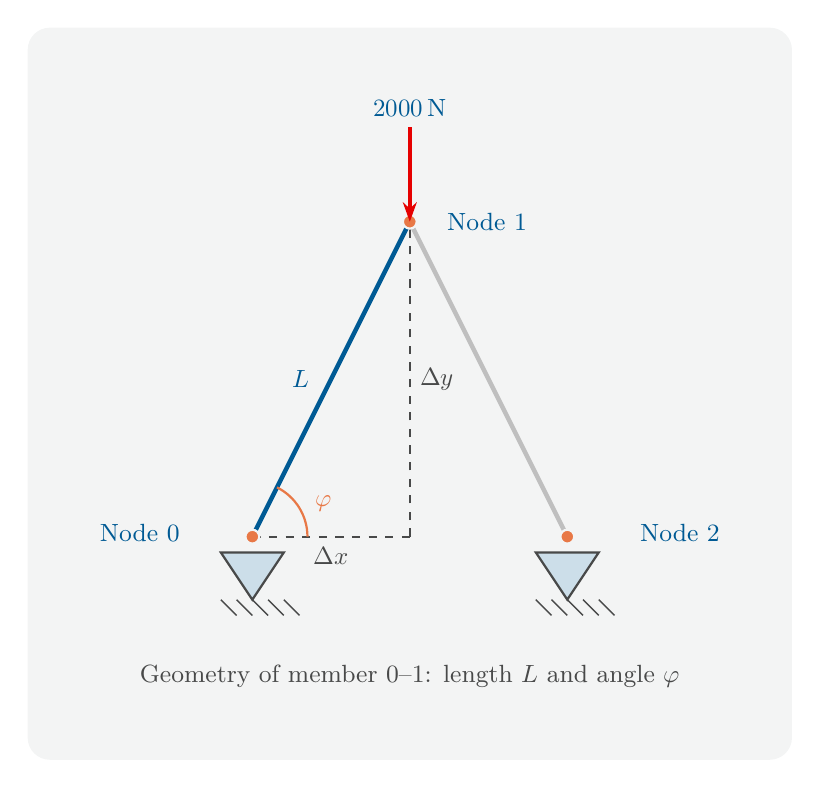
\begin{tikzpicture}[
    show background rectangle,
    background rectangle/.style={fill=my_lightgray, rounded corners=8pt},
    inner frame sep=0.8cm,
    annotation/.style={draw=my_darkgray, thick, -{Stealth[length=7pt, width=5pt]}}
]

    %------------------------------------------------------------
    % Knotenkoordinaten (skaliert mit Faktor 2)
    %------------------------------------------------------------
    \coordinate (N0)   at (0,0);
    \coordinate (N1)   at (2,4);
    \coordinate (N2)   at (4,0);
    \coordinate (Foot) at (2,0);   % Lotfußpunkt von N1 auf die x-Achse

    %------------------------------------------------------------
    % Stab 1-2: dezent grau (nicht im Fokus)
    %------------------------------------------------------------
    \draw[draw=my_darkgray!35, ultra thick] (N1) -- (N2);

    %------------------------------------------------------------
    % Stab 0-1: hervorgehoben (Fokus dieses Schritts)
    %------------------------------------------------------------
    \draw[draw=my_darkblue, ultra thick] (N0) -- (N1);

    %------------------------------------------------------------
    % Gestrichelte Hilfslinien: Δx und Δy (Komponenten des Differenzvektors)
    %------------------------------------------------------------
    \draw[dashed, draw=my_darkgray, thick]
        (N0) -- (Foot)
        node[midway, below, font=\small, text=my_darkgray] {$\Delta x$};
    \draw[dashed, draw=my_darkgray, thick]
        (Foot) -- (N1)
        node[midway, right, font=\small, text=my_darkgray] {$\Delta y$};

    %------------------------------------------------------------
    % Länge L als Beschriftung mittig auf dem Stab 0-1
    %------------------------------------------------------------
    \node[font=\small, text=my_darkblue, anchor=east]
        at ($(N0)!0.5!(N1)+(-0.15, 0.0)$) {$L$};

    %------------------------------------------------------------
    % Winkel φ als Kreisbogen an Knoten 0
    %------------------------------------------------------------
    \draw[draw=my_orange, thick]
        (0.7, 0) arc[start angle=0, end angle=63.43, radius=0.7];
    \node[font=\small, text=my_orange]
        at (0.9, 0.42) {$\varphi$};

    %------------------------------------------------------------
    % Knotenpunkte
    %------------------------------------------------------------
    \foreach \P in {N0, N1, N2} {
        \draw[fill=my_orange, draw=my_lightgray, thick] (\P) circle (2.5pt);
    }

    %------------------------------------------------------------
    % Lager an Knoten 0 (linkes Festlager)
    %------------------------------------------------------------
    \draw[fill=my_lightblue, draw=my_darkgray, thick]
        (-0.4,-0.2) -- (0.4,-0.2) -- (0,-0.8) -- cycle;
    \foreach \x in {-0.4,-0.2,0,0.2,0.4} {
        \draw[draw=my_darkgray, line width=0.5pt] (\x,-0.8) -- ++(0.2,-0.2);
    }

    %------------------------------------------------------------
    % Lager an Knoten 2 (rechtes Festlager)
    %------------------------------------------------------------
    \draw[fill=my_lightblue, draw=my_darkgray, thick]
        (4.4,-0.2) -- (3.6,-0.2) -- (4,-0.8) -- cycle;
    \foreach \x in {3.6,3.8,4.0,4.2,4.4} {
        \draw[draw=my_darkgray, line width=0.5pt] (\x,-0.8) -- ++(0.2,-0.2);
    }

    %------------------------------------------------------------
    % Äußere Last am freien Knoten 1
    %------------------------------------------------------------
    \draw[draw=my_red, ultra thick, -{Stealth[length=7pt, width=5pt]}]
        ($(N1)+(0,1.2)$) -- (N1);
    \node[font=\small, text=my_darkblue, anchor=south]
        at ($(N1)+(0,1.2)$) {$2000\,\mathrm{N}$};

    %------------------------------------------------------------
    % Knotenbeschriftungen
    %------------------------------------------------------------
    \node[font=\small, text=my_darkblue, anchor=east]
        at ($(N0)+(-0.8,0.05)$) {Node 0};
    \node[font=\small, text=my_darkblue, anchor=west]
        at ($(N1)+(0.35,0)$) {Node 1};
    \node[font=\small, text=my_darkblue, anchor=west]
        at ($(N2)+(0.8,0.05)$) {Node 2};

    %------------------------------------------------------------
    % Titel
    %------------------------------------------------------------
    \node[font=\small, text=my_darkgray, anchor=north]
        at (2,-1.5) {Geometry of member 0--1: length $L$ and angle $\varphi$};

\end{tikzpicture}
\end{document}